\def\baselinestretch{1}
\section{Test e risultati}
\def\baselinestretch{1.66}
\thispagestyle{headings}

\subsection{Test effettuati}
I risultati estratti da una shell dopo aver eseguito il programma prevedono vari grafi. Per ognuno
di essi vi sar\`a presente il grafico relativo.

\begin{center}
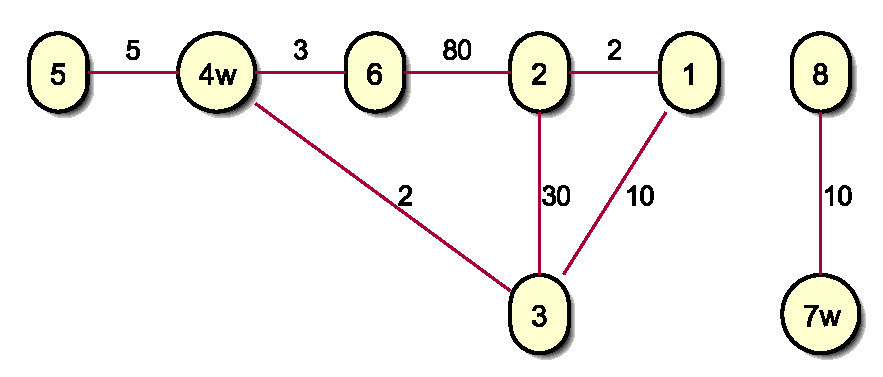
\includegraphics[scale=0.7]{tesina_tex/spacegraph/2img/notconn.eps}
\captionof{figure}{Grafo non connesso.}
\end{center}

\begin{minted}{bash}
Filling a graph with 8 nodes, 8 edges, 2 wormholes
STARTING READING FILE: 6
STARTING READING 2ndhalf: 2

Looking for a path from 1 to 8

Travel without wormholes: there are no paths that connect 1 with 8
        (disconnected graph)

Using wormholes -> [4, 7]: 1-3-4^7-8 in 23 unit time
\end{minted}

\newpage

\begin{center}
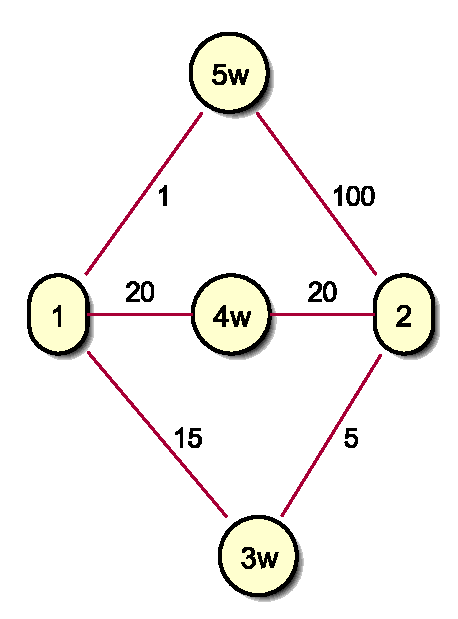
\includegraphics[scale=0.7]{tesina_tex/spacegraph/2img/diamond.eps}
\captionof{figure}{Grafo a diamante.}
\end{center}

\begin{minted}{bash}
Filling a graph with 5 nodes, 6 edges, 3 wormholes
STARTING READING FILE: 3
STARTING READING 2ndhalf: 3

Looking for a path from 1 to 2

Travel without wormholes: 1-3-2 in 20 time unit

Using wormholes -> [5, 3]: 1-5^3-2 in 7 unit time
\end{minted}



\newpage Nel grafo seguente il percorso con wormhole non \`e mostrato in quanto il wormhole
usato dalla sorgente e dalla destizione \`e lo stesso, infatti il nodo $11$ \`e presente
in entrambi i cammini minimi.
\begin{center}
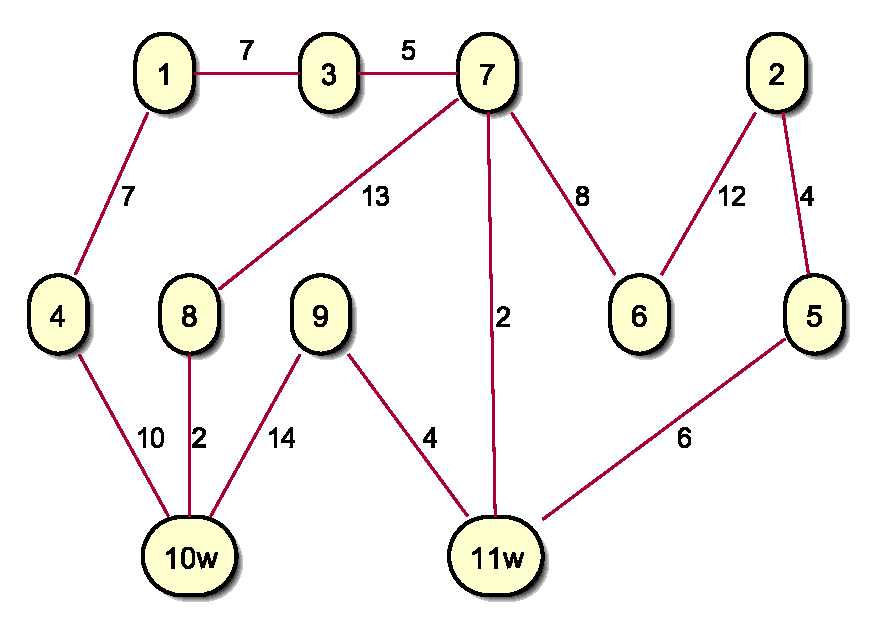
\includegraphics[scale=0.7]{tesina_tex/spacegraph/2img/traccia.eps}
\captionof{figure}{Grafo d'esempio.}
\end{center}

\begin{minted}{bash}
Filling a graph with 11 nodes, 13 edges, 2 wormholes
STARTING READING FILE: 11
STARTING READING 2ndhalf: 2

Looking for a path from 1 to 2

Travel without wormholes: 1-3-7-11-5-2 in 24 time unit

No fast travel with wormhole.
\end{minted}




\newpage Per puro stress testing del programma, si \`e utilizzato un file contentente
317080 nodi, 1049866 archi e 10 wormholes, ovviamente previo
commento nell'implementazione
del parser circa i controlli sull'input. Successimante si usa lo stesso file ma senza
wormhole in modo da non far applicare una seconda volta dijkstra.
Il risultato mostrato di seguito contiene l'esecuzione calcolandone i tempi tramite
l'applicativo \emph{time} presente nei sistemi operativi \emph{*NIX}

\begin{minted}[breaklines=true]{bash}
Filling a graph with 317080 nodes, 1049866 edges, 10 wormholes
STARTING READING FILE: 1049856
STARTING READING 2ndhalf: 10

Looking for a path from 316972 to 317029

Travel without wormholes:
316972-264079-298841-63506-59115-5530-26742-65338
-191800-287822-125483-121155-107180-308349-317029
in 104 time unit

Using wormholes -> [316972, 317029]: 316972^317029 in 1 unit time


real    1m42.700s
user    1m42.313s
sys     0m0.188s
\end{minted}
\newpage
Da notare come il file senza wormhole ci impiega circa la \textbf{met\`a}.

\begin{minted}[breaklines=true]{bash}
Filling a graph with 317080 nodes, 1049866 edges, 0 wormholes
STARTING READING FILE: 1049866
STARTING READING 2ndhalf: 0

Looking for a path from 316972 to 317029

Travel without wormholes:
316972-264079-298841-63506-59115-5530-26742-65338
-191800-287822-125483-121155-107180-308349-317029
in 104 time unit

No wormhole from Source to Destination.

real    0m56.303s
user    0m56.047s
sys     0m0.094s

\end{minted}

